\subsubsection{Key Storage} \label{section:counter-replace-encryption-key-online}
Decryption does not work without a decryption key.
This key has to be stored in a secure place since the encryption is only as strong as the protection of the key.

\subsubsection{Key Storage - Online and Caching} \label{section:counter-replace-encryption-key-online}
The first approach to handle the encryption key is to store it on a server and provide it to the application.
This works similar to the license verification.
\newline
On decrypt method call, the application tries to retrieve a cached cryptographic key.
In case a cached key is available, the application starts to decrypt the content.
Otherwise the key is requested from the server.
The server does a verification of the user similar to the license verification libraries.
In case the check is successful, the decryption key is sent to the device instead of a simple yes or no.
The advantage over having the original implementation is that the key can neither be accessed without the verification on the server nor guessed by an attacker to circumvent this countermeasure.
\newline
The key can either be retrieved from the server for each decryption action or it can be cached on the device, similar to the license verification policy.
Caching should be favored since getting the key for each action not only requires to be online but slows down the application and generates additional traffic.
\newline
In order to improve security, keys can be changed when updating the version of the application or be user specific.
\begin{figure}[h]
    \centering
    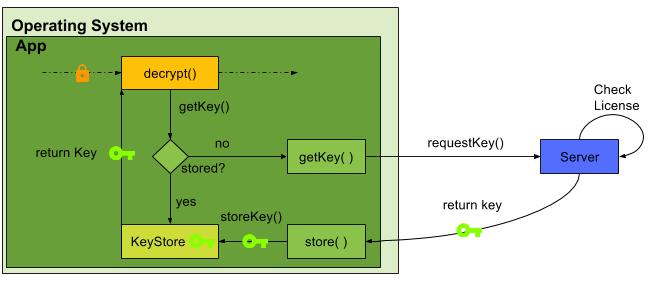
\includegraphics[width=0.8\textwidth]{data/encryptionKeyServer.png}
    \caption{Retrieving the key after successful identification from the server and store it local on device}
    \label{fig:encryptionKeyServer}
\end{figure}

\subsubsection{Key Storage - Secure Element} \label{section:counter-replace-encryption-key-local}
Since there are possibilities to read the cached key \cite{memoryDump} and crack the encryption this way, the use of a \gls{se} is proposed.
\newline
A secure element is a tamper-resistant platform which can be used to securely host applications and cryptographic keys \cite{seDefinition}.
There are different form factors for \gls{se}s \cite{seDefinition}.
For Android, the microSD is for Android the form factor of choice.
It can be either mounted in the microSD card slot or on the USB interface by using an adapter.
Using the USB interface requires the device to support \gls{otg} \cite{usbOtg}.
The \gls{se} is accessed over reads and writes to its filesystem.
Since the \gls{se} has to be small to fit the size of an microSD card and is powered by the host system, its hardware capabilities are constrained.
The result is a performance as low as 25MHz.
This does not allow complex computations on the \gls{se}. \cite{stSe}
For this reason the usage of the \gls{se} is restricted to simple tasks, like storing a key used for decryption.
The advantage of an \gls{se} is that its functionality is outside of the Android application and thus cannot be manipulated by \gls{luckypatcherg}.
\newline
An abstract presentation of the use of a \gls{se} can be seen in figure~\ref{fig:encryptionKeySmart}.
\newline
\begin{figure}[h]
    \centering
    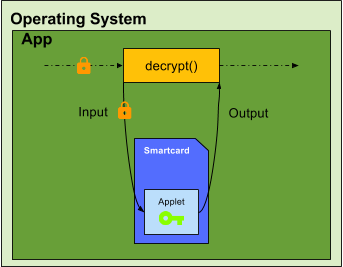
\includegraphics[width=0.8\textwidth]{data/encryptionKeySmart.png}
    \caption{Decryption by using a smartcard}
    \label{fig:encryptionKeySmart}
\end{figure}
At the moment, the integration of a \gls{se} comes with some problems.
\begin{itemize}
  \item the user has to buy extra hardware
  \item not all devices have a microSD card slot or support \gls{otg}
  \item no unified implementations for communication with the \gls{se} across manufacturers
\end{itemize}
The first problem is that the user has to buy extra hardware.
This means extra money has to be spend and the hardware has to be always around.
In addition, the connection to the device using a cable is not the most convenient solution.
/newline
The second problem is that some devices neither have an microSD card slot nor implemented \gls{otg} support.
For example, the Nexus 7 (2012) and the Nexus 6P neither have the capability to use a microSD card.
While the Nexus7 was supposed to have \gls{otg}, it did not work with the used \gls{se}, while the Nexus 6P did not support \gls{otg} out of the box.
Both devices needed even needed additional plugins to read the \gls{otg} mounted microSD in a file explorer.
The third problem is that each manufacturer implements its own interpretation for the interface which makes \gls{se} incompatible to each other.
For this reason, the SD Association proposed the smartSD in order to have a universal standard for \gls{se}s \cite{smartSD}.
